\documentclass{amsart}
\usepackage{amssymb}
\usepackage{color}
\usepackage{tikz}
\usetikzlibrary{trees,arrows}
\usetikzlibrary{patterns}
\usetikzlibrary{positioning}
\tikzset{mynode/.style={draw,text width=4cm,align=center}
}
\usepackage{tkz-fct,tkz-euclide,tikz-layers}
\tikzset{arrow coord style/.style={dotted, opacity=.8, thin}}
\tikzset{xcoord style/.style={
		font=\footnotesize,text height=1ex,
		inner sep = 0pt,
		outer sep = 0pt,
		text=black}}
\tikzset{ycoord style/.style={
		font=\footnotesize,text height=1ex,
		inner sep = 0pt,
		outer sep = 0pt,
		text=black}}

\newcommand{\BR}{{\mathbb R}}

\begin{document}

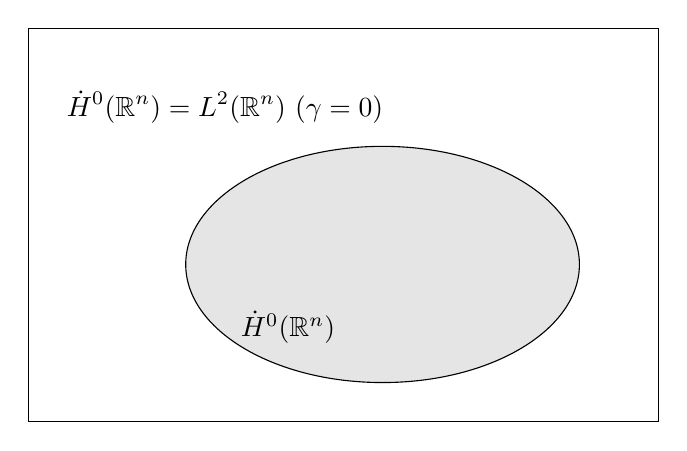
\begin{tikzpicture}
		\draw (0,0) rectangle (8,5);  
		\node [at={(2.5,4)}] {$\displaystyle \dot{H}^{0}(\BR^n)=L^2(\BR^n)$~$(\gamma=0)$};
		\draw[fill=gray!20] (4.5,2) ellipse[x radius = 2.5, 
		y radius = 1.5];
		\node [at={(3.3,1.2)}] {$\dot{H}^{0}(\BR^n)$};
	\end{tikzpicture}

\end{document}